\chapter{Koch Snowflake}

\noindent Koch Snowflake është një shembull klasik i një fraktali, i përshkruar për herë të parë nga matematikani suedez Heldge von Koch në vitin 1904. Fraktali mund të konstruktohet duke filluar nga një trekëndësh barabrinjës, dhe pastaj rekursivisht duke ndryshuar çdo segment si vijon:

\begin{enumerate}
    \item ndaj segmentin në tri pjesë të barabarta.
    \item ndërto një trekëndësh barabrinjës me bazë segmentin e mesëm të fituar nga hapi i parë.
    \item largo segmentin e mësëm  që është baza e trekëndëshit nga hapi i dytë.
\end{enumerate}

\noindent Katër iterimet e para të këtij fraktali janë paraqitur në  figurën \ref{fig:koch_4}. Me rritjen e iterimeve do të fitohet figura \ref{fig:koch_big}.

\begin{figure}[htbp!]
\hfill
\subfigure[iterimi 0]{\includegraphics[width=0.22\linewidth]{koch_1}}
\hfill
\subfigure[iterimi 1]{\includegraphics[width=0.22\linewidth]{koch_2}}
\hfill
\subfigure[iterimi 2]{\includegraphics[width=0.22\linewidth]{koch_3.png}}
\hfill
\subfigure[iterimi 3]{\includegraphics[width=0.22\linewidth]{koch_4.png}}
\hfill
\caption{Koch Snowflake në iterimet e para.}
\label{fig:koch_4}
\end{figure}

\section{Konstruktimi i trekëndëshit barabrinjës}

\noindent Le të jenë dhënë pikat \( A(x_1, y_1) \) dhe \( B(x_2, y_2) \). Duhet të gjejmë pikat \( C \), \( D \), \( E \) ashtuqë 
\( \overrightarrow{AC} = \frac{1}{2} \overrightarrow{CB} \), \( \overrightarrow{DB}=\frac{1}{2}\overrightarrow{AD}\), dhe trekëndëshi \( \triangle CDE \) të jetë barabrinjës (fig \ref{fig:koch_construction}). \\

\noindent Nga barazimi \( \overrightarrow{AC} = \frac{1}{2} \overrightarrow{CB} \), marrim

\[ 
\left( c_1 - x_1, c_2 - y_1 \right) = \frac{1}{2} \left( x_2 - c_1, y_2 - c_2 \right) 
\]

\begin{figure}
    \centering
    \includegraphics[width=1\linewidth]{koch_5.png}
    \caption{Konstruktimi i trekëndëshit.}
    \label{fig:koch_construction}
\end{figure}

\noindent \\ Duke barazuar kordinatat përkatëse të dysheve të renditura në të dy anët e barazimit, marrim

\[
(c_1 - x_1) = \frac{1}{2} (x_2 - c_1)
\]
\[
(c_2 - y_1) = \frac{1}{2} (y_2 - c_2)
\]

\noindent Dhe fitojmë kordinatat e pikës \( C = (c_1, c_2) = \left( \frac{x_2 - 2x_1}{3}, \frac{y_2 - 2y_1}{3} \right) \). Në mënyrë analoge gjenden edhe kordinatat e pikës \( D \).

\noindent \\ Trekëndëshi \( \triangle CDE \) është barabrinjës dhe rrjedhimisht çdo kënd i tij është 60 shkallë. Mjafton ta rrotullojmë pikën \( D \) rreth pikës \( C \) për 60 shkallë për të fituar pikën \( E \). 

\[
e_1 = (d_1 - c_1) \cos\left(\frac{\pi}{3}\right) - (d_2 - c_2) \sin\left(\frac{\pi}{3}\right) + c_1
\]

\[
e_2 = (d_1 - c_1) \sin\left(\frac{\pi}{3}\right) + (d_2 - c_2) \cos\left(\frac{\pi}{3}\right) + c_2
\]

\noindent \\ Nëse këndin e rrotullimit e marrim \(-60\) shkallë, atëherë do të fitojmë fraktalin Koch Anti-Snowflake e paraqitur në figurën \ref{fig:koch_anti}.
\section{Numri i pikave} 

Shënojmë me \( f(n) \) numrin total të pikave të figurës në iterimin  \( n \). Në iterimin 0 kemi tre pika, dhe pas secilit iterim në secilën brinjë shtohen nga tre pika.

\[
f(0) = 3
\]

\[
f(1) = 3f(0) + f(0) = 4f(0) = 4 \times 3
\]

\[
f(2) = 3f(1) + f(1) = 4f(1) = 4^2 \times 3
\]

\[
f(3) = 3f(2) + f(2) = 4f(2) = 4^3 \times 3
\]

\[
\vdots
\]

\[
f(n) = 3 \times 4^n
\]

\noindent Këtë varg e përdorim për të i treguar OpenGL, se sa pika do i bashkoj si segmente, pasi kemi llogaritur kordinatat e pikave të figurës(rreshti 6). \\

\begin{lstlisting}
void renderSnowflakeFromBuffer() {
    glColor3f(0.29f, 0.44f, 0.55f);
    glPointSize(7.0f);
    glVertexAttribPointer(0, 2, GL_FLOAT, GL_FALSE, 0, nullptr);
    glEnableVertexAttribArray(0);
    numberOfPoints = 3*pow(4, iterations);
    glDrawArrays(GL_LINE_LOOP, 0, numberOfPoints);
}
\end{lstlisting}

\section{Paralelizimi}

\noindent Paralelizimi ndodh në menyrë hiearkike, ku në secilin iterim do të jenë aktiv një numër i caktuar i thredave. Secili thread aktiv do e marë brinjën e 
\(i\) - të të figurës, dhe do të i gjejë tre pikat për ndërtimin të trekëndëshit mbi segment. Katër segmentet e gjetura secili thread do i fut në vargun e të gjitha brinjëve. Ky varg përmban të gjitha brinjët e gjeneruara për secilin iterim, dhe madhësia e tij është:
\[
h(n) = f(0) + f(1) + \cdots + f(n-1) = \sum_{i=0}^{n-1} f(i) = 3 \sum_{i=0}^{n-1} 4^i = 4^n - 1
\]

\noindent Për secilin iterim do të jenë \( 3 \times 4^n \)  threada aktiv për gjetje të pikave të reja. Me rritje të iterimeve, numri i threadave aktiv do të ngritet eksponencialisht.

\begin{enumerate}
\item Iterimi 0: Vetëm threadi me id 0 të jetë aktiv. Ky thread inicalizon trekëndëshin fillestar.
\item Iterimi 1: Threadat 1-3 janë aktiv. Secili thread mer segmentin përkatës të trekëndëshit fillestar dhe ndërton trekëndëshin barakrahësh në të.   
\item Iterimi 2: 4-15 janë aktiv. Këta threada marrin segmentet nga iterimi i kaluar dhe ndërtojnë trekëndësha barakrahësh në ta.
\item Iterimi n: Threadat \(4^{n-1}\) deri në \(4^n-1\) do të jenë aktiv. Këta threada marin segmentet nga iterimi i kaluar dhe ndërtojnë trekëndëshat barakrahësh në ta. 

\end{enumerate}

\noindent Kjo qasje hiearkike siguron që secili iterim të shfrytëzojë fuqinë e plotë të përpunimit paralel. Në figurën \ref{fig:koch_threads} është vizualizuar ky proces i threadave. Vijat me ndërpreje nënkuptojnë se se threadat janë duke pritur që të mbërrihet iterimi i ardhshëm për tu bërë aktiv.

\begin{figure}[!]
    \centering
    \includegraphics[width=1\linewidth]{koch_6.png}
    \caption{Sinkronizimi dhe ekzekutimi paralel.}
    \label{fig:koch_threads}
\end{figure}


\section{Kerneli}

Kerneli i mëposhtëm gjeneron fraktalin përmes llogaritjes paralele. Fillimisht threadi me indeks 0 trajton trekëndëshin inicializues. Për secilin iterim threads ndërmjet intervalit start\_at dhe end\_at janë aktiv dhe llogaritin pikat e nevojshme për të formuar lakorën Koch. Rezultatet ruhen në vargun e segmenteve dhe kulmet i shtohen vargut points për vizualizim. Sinkronizimi siguron që të gjitha threadat përfundojnë detyrën e tyre para sa te të vazhdojnë në iterimin e ardhshëm. \\


\begin{lstlisting}
__global__ void kernel(float* points, Segment* segments, int start_iteration, int max_iteration	, int inverted, int threadShiftIndex) {
    Point A,B,C,A1,B1,C1;
    Segment segment_1, segment_2, segment_3, segment_4;
    
    int idx = threadIdx.x + blockIdx.x * blockDim.x;
    idx += threadShiftIndex;
    
    if (idx == 0) {
    //CODE to handle the first iteration
    }

    auto g = cg::this_grid();
    __syncthreads();

    for (int iteration = start_iteration; iteration <= max_iteration; iteration++){
        int start_at = pow(4.0, iteration - 1);
        int end_at = pow(4.0, iteration);
        if (idx >= start_at && idx < end_at) {
              //Segment to built Koch curve on
            Segment segment = segments[idx];
            A = segment.A;
            B = segment.B;
            triangleOnSegment(A, B, &A1, &B1, &C1, inverted);
            //Koch curve
            segment_1.A = A;
            segment_1.B = B1;
            segment_2.A = B1;
            segment_2.B = C1;
            segment_3.A = C1;
            segment_3.B = A1;
            segment_4.A = A1;
            segment_4.B = B;
            //Insert the generated koch curvers into segments array
            int offset = end_at + 4 * (idx - start_at);
            segments[offset] = segment_1;
            segments[offset + 1] = segment_2;
            segments[offset + 2] = segment_3;
            segments[offset + 3] = segment_4;
            //Insert vertices to points array
            offset = 2 * 4 * (idx - start_at);
            points[offset] = A.x;
            points[offset + 1] = A.y;
            points[offset + 2] = B1.x;
            points[offset + 3] = B1.y;
            points[offset + 4] = C1.x;
            points[offset + 5] = C1.y;
            points[offset + 6] = A1.x;
            points[offset + 7] = A1.y;
            points[offset + 8] = B.x;
            points[offset + 9] = B.y;
        }
        g.sync();
    }
}

\end{lstlisting}

\section{Krahasimet}

\noindent Tabela \ref{tab:koch_tab} krahason kohën e ekzekutimit në mikrosekonda të fraktalit ndërmjet versionit sekuencial dhe të versionit paralel. Implementimi me CUDA është bërë me  anë të grupeve kooperative, me 23040 threada për një thirrje të kernelit. Vizualizimi i këtyre rezultave është në figurën \ref{fig:koch_graph}.

% Please add the following required packages to your document preamble:
% \usepackage{booktabs}
% \usepackage{graphicx}
% Please add the following required packages to your document preamble:
% \usepackage{graphicx}
\begin{table}[h]
\centering
\resizebox{0.3\textwidth}{!}{%
\begin{tabular}{|l|l|l|}
\hline
Iterimi & C++ & CUDA \\ \hline
0 & 2 & 23 \\ \hline
1 & 3 & 26 \\ \hline
2 & 16 & 41 \\ \hline
3 & 17 & 29 \\ \hline
4 & 50 & 37 \\ \hline
5 & 140 & 25 \\ \hline
6 & 787 & 27 \\ \hline
7 & 2514 & 60 \\ \hline
8 & 9101 & 93 \\ \hline
9 & 37411 & 409 \\ \hline
10 & 154053 & 1384 \\ \hline
11 & 607546 & 5032 \\ \hline
12 & 2240534 & 326359 \\ \hline
13 & 9075431 & 3123194 \\ \hline
\end{tabular}%
}
\caption{Krahasimi i performancës.}
\label{tab:koch_tab}
\end{table}




\begin{figure}[htpb]
\centering
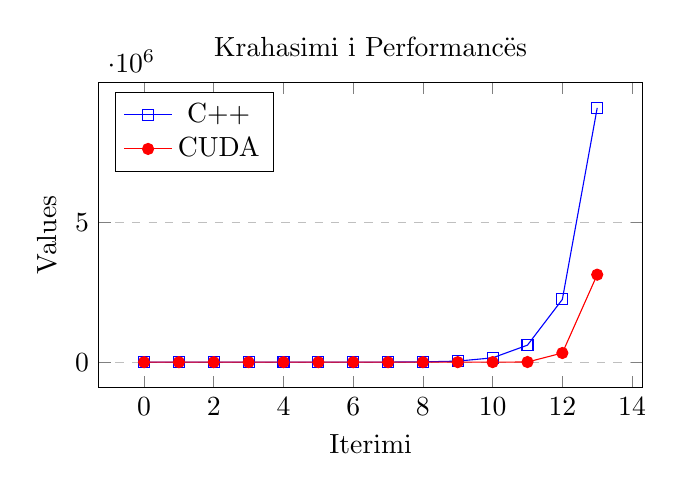
\begin{tikzpicture}
\begin{axis}[
    title={Krahasimi i Performancës},
    xlabel={Iterimi},
    ylabel={Values},
    legend pos=north west,
    ymajorgrids=true,
    grid style=dashed,
    width=0.7\textwidth,  % Adjusted width
    height=0.45\textwidth, % Adjusted height
]
\addplot[
    color=blue,
    mark=square,
    ]
    coordinates {
    (0,2)(1,3)(2,16)(3,17)(4,50)(5,140)(6,787)(7,2514)(8,9101)(9,37411)(10,154053)(11,607546)(12,2240534)(13,9075431)
    };
\addplot[
    color=red,
    mark=*,
    ]
    coordinates {
    (0,23)(1,26)(2,41)(3,29)(4,37)(5,25)(6,27)(7,60)(8,93)(9,409)(10,1384)(11,5032)(12,326359)(13,3123194)
    };
\legend{C++, CUDA}
\end{axis}
\end{tikzpicture}
\caption{Grafiku i krahasimit të performancës.}
\label{fig:koch_graph}
\end{figure}

\newpage

\begin{figure}[htp]
\centering
\subfigure[Koch Snowflake\label{fig:koch_snowflake_13}]{\includegraphics[width=0.8\linewidth]{koch_7.png}}
\subfigure[Koch Anti-Snowflake]{\label{fig:koch_anti}\includegraphics[width=0.8\linewidth]{koch_8.png}}
\caption{Fraktali në iterimin 11 i gjeneruar me CUDA.}
\label{fig:koch_big}
\end{figure}


% \begin{figure}[htp]
% \begin{figure}
%     \centering
%     \includegraphics[width=1\linewidth]{koch_8.png}
%     \caption{Enter Caption}
%     \label{fig:enter-label}
% \end{figure}
%     \centering
%     \includegraphics[width=0.6\linewidth]{koch_8.png}
%     \caption{Enter Caption}
%     \label{fig:enter-label}
% \end{figure}

